% !TEX root = ../report.tex

\section{Logical View}
\label{sec:viewlogical}

% Logical view : The logical view is concerned with the functionality that the system provides to end-users. UML Diagrams used to represent the logical view include Class diagram, Communication diagram, Sequence diagram.

Docker is made using the the go language created by Google. Docker is an application categorized as ``Operating-system-level virtualization''. It consists of:
\begin{itemize}
\item 2979205 lines of go code (almost 3 million).
\item 1782 '.go' files
\item 267 different packages
\end{itemize}

If the main ``/docker'' package is build, the dependencies can be visualized using a  visualization tool. When restricting the depth to be 1, it produces the image below, Figure \ref{fig:dockerdep1}. The green node is the "main" node for which the dependencies are shown.

\begin{figure}[H]
\caption{A high-level overview of the Docker architecture.}
\centering
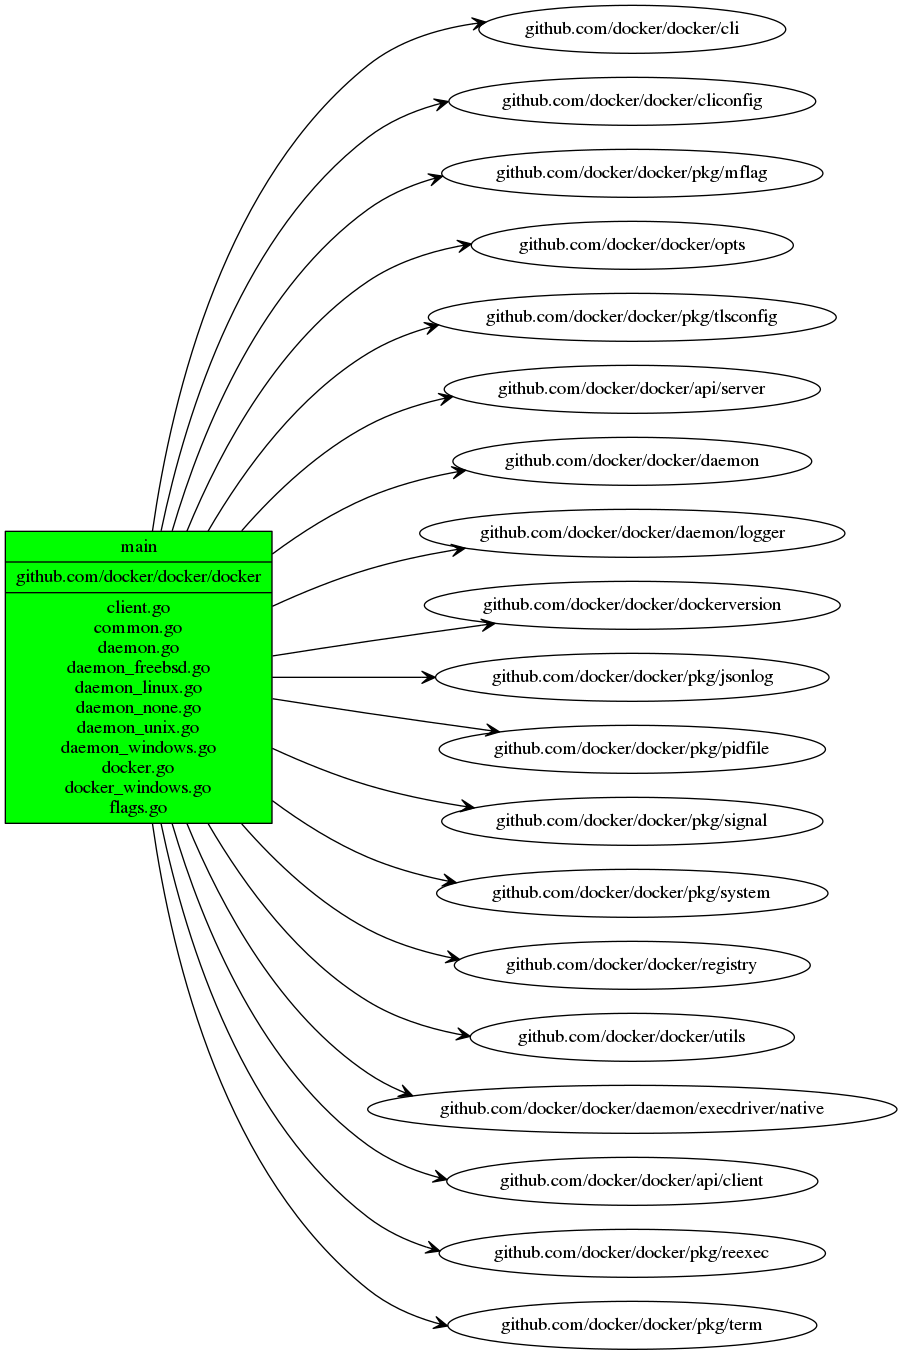
\includegraphics[width=\linewidth, height=15cm]{images/dependencyGraphs/goviz/govizgreendocker1.png}
\label{fig:dockerdep1}
\end{figure}

Looking at the official documentation, their image (Figure \ref{fig:dockerarchipic}) shows to be largely similar.\\

\begin{figure}[H]
\caption{A high-level overview of the Docker architecture. Source: \cite{dockerarchi}.}
\centering
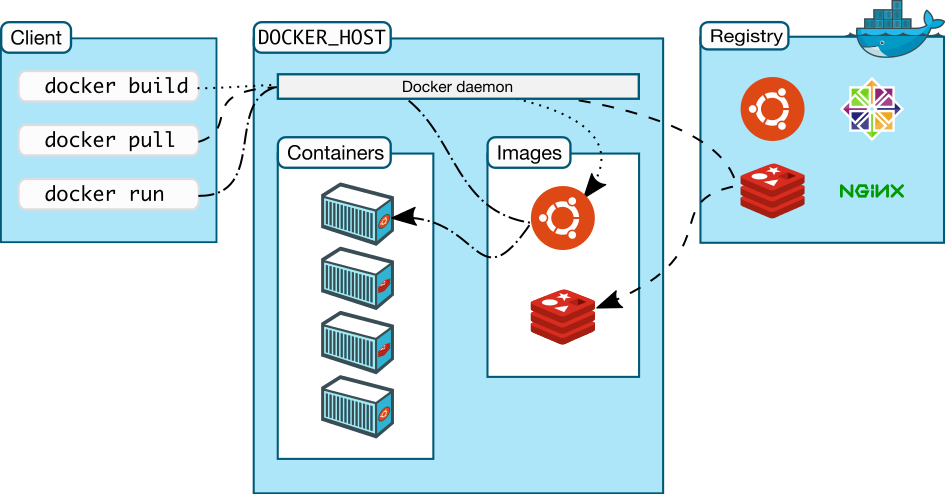
\includegraphics[scale=0.4]{4-softwarearch/images/architecture.png}
\label{fig:dockerarchipic}
\end{figure}
Docker uses a client-server architecture. The client (a command-line tool) acts as the primary user interface and talks to the Docker daemon. The daemon is a background process which does all the heavy lifting, e.g. the building and running of the containers.


%TODO Research about the importance of the packages will be added still...
The most important part of docker will be discussed in the following sections below.

\subsection{Client}
The client is a small binary and acts as the primary user interface to Docker. The user enters commands into the client and the client forwards these commands to the Docker daemon, which executes commands.
The Docker client is capable of connecting to daemons running on the local machine, as well as connecting to daemons running on remote machines over the internet.

\subsection{Server / Daemon}
The Docker daemon is a process running on the host machine (as can be seen in Figure~\ref{fig:dockerarchipic}). This process is usually started when the host machine starts and runs in the background. It exposes a REST interface and listens for requests coming from clients on the same or remote hosts.

\subsubsection{Images}
Docker images can be interpreted as a read-only template from which Docker containers are
started. A Docker image consists of a stack of layers which are bonded by a union
file system. These layers support reusability and sharing.

Docker images can be built from text files (`Dockerfiles'), which contain instructions like installing software and copying files.

\subsubsection{Containers}
% running usin libcontainer from the open specification
Docker containers are based on Docker images. These images consist of read-only
layers. Then, for a Docker container, a thin writable layer is added on top of it to
perform operations. Docker containers basically consist of the files of the operating system,
user-added files, application files, and data files. Multiple containers may run
based on the same image. In this case, Docker will not create separate copies for
each containers. Instead, they will share the same image with their own writable
layer.

To run Docker containers, Docker uses the \verb|libcontainer| library, which is part of the Open Container Initiative.

\subsection{Registry}
A Docker registry is a place where Docker images can be stored and retrieved. The Docker daemon
fetches desired Docker images from this repository. This registry may be a
public or a private one, such as one behind a firewall. Docker
Hub\footnote{\url{https://hub.docker.com/}} is one example of a docker registry
hosted by Docker. A registry provides an easy way to distribute images among different hosts.
